\documentclass{paper}

%\usepackage{times}
\usepackage{epsfig}
\usepackage{graphicx}
\graphicspath{{superresolution/}{superresolution/output/}}
\usepackage{amsmath}
\usepackage{amssymb}
\usepackage{color}
\usepackage{hyperref}
\usepackage[tight,footnotesize]{subfigure}

% load package with ``framed'' and ``numbered'' option.
%\usepackage[framed,numbered,autolinebreaks,useliterate]{mcode}

% something NOT relevant to the usage of the package.
\setlength{\parindent}{0pt}	
\setlength{\parskip}{18pt}
\newcommand{\prox}{\text{prox}}
\newcommand{\norm}[1]{\left\lVert#1\right\rVert}
\newcommand{\twonorm}[1]{\left\lVert#1\right\rVert_2}
\usepackage[latin1]{inputenc} 
\usepackage[T1]{fontenc} 

\usepackage{listings} 
\lstset{% 
   language=Matlab, 
   basicstyle=\small\ttfamily, 
} 

\title{Assignment 2}



\author{Moser Stefan\\09-277-013}
% //////////////////////////////////////////////////


\begin{document}



\maketitle


% Add figures:
%\begin{figure}[t]
%%\begin{center}
%\quad\quad   \includegraphics[width=1\linewidth]{ass2}
%%\end{center}
%
%\label{fig:performance}
%\end{figure}

\section*{Superresolution}

\subsection*{Primal Dual formulation}
The energy term we need to minimize for this problem is

\begin{equation}
\min_{u \in U} \norm{\nabla u} + \frac{\lambda}{2} \twonorm{Du - g}^2
\label{eq:initial_energy}
\end{equation}
with $D$ being the downsampling operator that produces from the high 
resolution image $u$ (of size $M \times N$) a low level resolution image
(of size $\frac{M}{\alpha} \times \frac{N}{\alpha}$) by multiplying. 
For all images, we assume that they are given as vectors\footnote{following the flattening conventions of matlabs $(:)$ operator}.

So far, everything is the same as in the previous exercise. But instead of
solving Equation \eqref{eq:initial_energy} directly, we will derive the primal-dual
formulation
\begin{equation}
\min_{u \in U} \max_{y \in Y} < Ku, y > - F^*(y) + G(u)
\label{eq:dual_energy}
\end{equation}
and solve it instead. All needed conditions are met:
\begin{itemize}
\item $F = \norm{\cdot}_2$ is a convex function
\item $G = \frac{\lambda}{2}\twonorm{ D\cdot - g}^2$ is a convex function
\item $K = \nabla \cdot$ is a linear operator
\end{itemize}
\subsubsection*{Legendre Fenchel Transform of TV term}
Since $F$ only appears as it's convex conjugate $F^*$ in Equation \eqref{eq:dual_energy}, we need to compute it first.
\begin{align}
	F^*(y) &= (\norm{\cdot}_2)^*(y) \\
		  &= \sup_x x^T y - \twonorm{x} \\
		  &= \sup_x x^T y - \max_{\twonorm{z} \leq 1} x^T z \label{eq:cauchy_schwarz}\\
		  &= \sup_x \min_{\twonorm{z} \leq 1} x^T(y-z) \\
		  &= \begin{cases}
   				0  			& \text{if} \twonorm{y} \leq 1 \\
   				\infty      & \text{otherwise}
  			 \end{cases} \label{eq:cases_F_star} \\
  	      &= \delta(y)
\end{align}
In step \eqref{eq:cauchy_schwarz} we used the Cauchy-Schwarz inequality
\begin{equation}
	\twonorm{x} = \max_{\twonorm{z} \leq 1} x^T z
\end{equation}
Further, the result in Equation \eqref{eq:cases_F_star} can be derived by seeing that 
the inner minimum term always will be 0 in the first case, since then z will adapt to be
equal to y, resulting in the multiplication with a zero vector. If z can not be set equal
to y, i. e. $\twonorm{y} > 1$, the superior is unbound.

Consequently, the convex conjugate of the two norm is the \emph{unit ball indicator function}\footnote{1 if inside, $\infty$ if outside}.

We arrive at the Primal-Dual formulation for super resolution by simply putting our
results so far into Equation \eqref{eq:dual_energy}.
\begin{equation}
\min_{u \in U} \max_{y \in Y} <\nabla u, y> - \delta(y) + \frac{\lambda}{2}\twonorm{Du - g}^2
\end{equation}

\subsection*{Primal-Dual steps}
Equation \eqref{eq:dual_energy} can be solved using Primal-Dual steps. Specifically,
the following algorithm:
\begin{align}
	y^{n+1} &= \prox_{\sigma F^*}(y^n + \sigma K \bar{x}^n) \label{eq:yn1} \\
	x^{n+1} &= \prox_{\tau G}(x^n + \tau K^* y^{n+1}) \label{eq:xn1} \\
	\bar{x}^{n+1} &= x^{n+1} + \theta(x^{n+1} - x^n) \label{ex:barxn1}
\end{align}
with $\theta \in (0, 1]$ and $\tau \sigma \norm{K}^2 < 1$. 

The proximity operator used there is defined as 
\begin{equation}
	\prox_{\lambda F}(z) = \arg \min_x \frac{1}{2} \twonorm{x - z}^2 + \lambda F(x)
\end{equation}
The terms from Equation \eqref{eq:xn1} and \eqref{eq:yn1} need some further derivation
before they can be used, which is done in the following.

\subsubsection*{Derivation of $y^{n+1}$}
For the first term defined in Equation \eqref{eq:yn1} we get the following derivation:
\begin{align}
	y^{n+1} &= prox_{\sigma F^*}(y^n + \sigma K \bar{x}^n) \\
			&= y^n + \sigma K \bar{x}^n - 
				\sigma \cdot \prox_{F / \sigma}((y^n + \sigma K \bar{x}^n) / \sigma) 
				\label{eq:moreaus_identity_used} \\
			&= y^n + \sigma \nabla \bar{x}^n - 
				\sigma \cdot \prox_{\twonorm{\cdot} / \sigma}((y^n + \sigma \nabla \bar{x}^n) / \sigma)
				\label{eq:two_norm_proximity_used}
\end{align}
using Moreau's Identity in step \eqref{eq:moreaus_identity_used} which is defined as
\begin{equation}
	\prox_{\lambda F^*}(z) = z - \lambda \cdot \prox_{F/ \lambda}(z / \lambda) 
\end{equation}
Now, we need to compute the proximity operator of the two norm as it 
occurs in Equation \eqref{eq:two_norm_proximity_used} TODO: either fully derive or delete.
\begin{align}
	\prox_{\twonorm{\cdot} / \lambda}(z / \lambda) 
	&= \arg \min_x \frac{1}{2} \twonorm{x - \frac{z}{\lambda}}^2 +
	\frac{1}{\lambda} \twonorm{x} \\
	\label{eq:P_x}
	&= \arg \min_x P(x)
\end{align}
This can be solved by deriving and setting to zero:
\begin{align}
\frac{\partial}{\partial x} P(x) &= 
	\frac{\partial}{\partial x} \left(
 		\frac{1}{2} \twonorm{x - \frac{z}{\lambda}}^2 +
		\frac{1}{\lambda} \twonorm{x} 
	\right) \\
&= 
	\frac{\partial}{\partial x} \left(
		\frac{1}{2} (x-\frac{z}{\lambda}) (x-\frac{z}{\lambda}) + 
		\frac{1}{\lambda} (x^2)^{\frac{1}{2}}
	\right) \\
&= 
	x-\frac{z}{\lambda} + 
	\frac{\partial}{\partial x} \left(
		\frac{1}{\lambda} (x^2)^{\frac{1}{2}}
	\right) \\
&= 
	x-\frac{z}{\lambda} + 
	\frac{1}{\lambda} 2x \frac{1}{2} (x^2)^{-\frac{1}{2}} \\
&= 
	x-\frac{z}{\lambda} + 
	\frac{1}{\lambda} \frac{x}{\twonorm{x}} \overset{!}{=} 0 
	\label{eq:proximity_operator_l2_norm_fail}
\end{align}
Since we can not easily solve Equation \eqref{eq:proximity_operator_l2_norm_fail} for $x$, we need to express $P(x)$ as defined in \eqref{eq:P_x} in a more convenient form.
\begin{align}
todo
\end{align}
So we end up with
\begin{equation}
	\prox_{\twonorm{\cdot} / \lambda}(z / \lambda) =
	z / \lambda \cdot \max \left(0 , 1 - \frac{1}{\twonorm{z}} \right)
\end{equation}
Plugging this into Equation \eqref{eq:two_norm_proximity_used}, we get
\begin{align}
	y^{n+1} &= y^n + \sigma \nabla \bar{x}^n - 
			   \sigma \cdot ((y^n + \sigma \nabla \bar{x}^n) / \sigma \cdot
			   \max \left(0, 1 - \frac{1}{\twonorm{y^n + \sigma \nabla \bar{x}^n)}} \right) \\
			&= y^n + \sigma \nabla \bar{x}^n - 
			   (y^n + \sigma \nabla \bar{x}^n) \cdot
			   \max \left(0, 1 - \frac{1}{\twonorm{y^n + \sigma \nabla \bar{x}^n)}} \right) \\
			&= \begin{cases}
   				y^n + \sigma \nabla \bar{x}^n  			
   						& \text{if} \twonorm{y^n + \sigma \nabla \bar{x}^n)} \leq 1 \\
   				\frac{y^n + \sigma \nabla \bar{x}^n}
				    {\twonorm{y^n + \sigma \nabla \bar{x}^n}}      
				    		& \text{otherwise}
  			 \end{cases} \\
			&= \frac{y^n + \sigma \nabla \bar{x}^n}
				    {\max \left(1, \twonorm{y^n + \sigma \nabla \bar{x}^n}\right)}
\end{align}

\subsubsection*{Derivation of $x^{n+1}$}
The derivation of the second term (Equation \eqref{eq:xn1}) is similar 
to the one in the last section. 
\begin{align}
x^{n+1} &= \prox_{\tau G}(x^n + \tau K^* y^{n+1}) \\
	    &= \prox_{\tau \frac{\lambda}{2}\twonorm{ D\cdot - g}^2}(x^n + \tau \nabla^* y^{n+1}) \\
	    &= \arg \min_m \frac{1}{2} \twonorm{m - x^n + \tau \nabla^* y^{n+1}}^2 + \tau \frac{\lambda}{2}\twonorm{ Dm - g}^2 \\
	    &= \arg \min_m L(m)
\end{align}
The extrema of $L(m)$ can be found by setting the derivative 
with respect to m to zero. Since it is a convex function, we can be sure that the 
found value is the minimum.
\begin{align}
\frac{\partial}{\partial m} L(m) &= \frac{\partial}{\partial m} \left( \frac{1}{2} \twonorm{m - x^n + \tau \nabla^* y^{n+1}}^2 
+ \tau \frac{\lambda}{2}\twonorm{ Dm - g}^2 \right) \\
&= m - x^n + \tau \nabla^* y^{n+1} +
\frac{\partial}{\partial m} \tau \frac{\lambda}{2}\twonorm{Dm - g}^2 \\
&= m - x^n + \tau \nabla^* y^{n+1} +
\tau \lambda D(m - g) \\
&= m - x^n + \tau \nabla^* y^{n+1} +
\tau \lambda Dm - \tau \lambda D g \\
&= (I + \tau \lambda D)m - x^n + \tau \nabla^* y^{n+1} +
\tau \lambda D g \overset{!}{=} 0 \\
\Longleftrightarrow m &= (I + \tau \lambda D)^{-1} 
(x^n - \tau \nabla^* y^{n+1} + \tau \lambda D g)
 \\
&=  (I + \tau \lambda D)^{-1} (x^n + \tau \nabla y^{n+1} + \tau \lambda D g) \\
&= x^{n+1}
\end{align}

\subsubsection*{Overview of Primal-Dual steps}
After derivation, we have the following steps:
\begin{align}
y^{n+1} &= \frac{y^n + \sigma \nabla \bar{x}^n}
				{\max \left( 1, \twonorm{y^n + \sigma \nabla \bar{x}^n} \right)} \\
x^{n+1} &= (I + \tau \lambda D)^{-1} 
           (x^n + \tau \nabla \cdot y^{n+1} + \tau \lambda D g) \\
\bar{x}^{n+1} &= x^{n+1} + \theta(x^{n+1} - x^n)
\end{align}
and are ready for doing our implementation.

\subsection*{Implementation}
I chose the following parameters for my implementation
\begin{align}
	K_a 	&= 8 \\
	\sigma 	&= 0.001 \\
	\tau  	&= \frac{1}{K_a \cdot \tau}
	\label{eq:tau}
\end{align}
\subsubsection*{Iteration count}
The number of iterations needed is heavily dependent on lambda. 
Smaller lambdas need much longer to converge than larger ones. 
The behavior of the energy function for both cases is visible in Figure \ref{fig:energy_plots}. 
Some intermediary images for a small lambda can be seen in Figure \ref{fig:iteration_count_lambda_50}, for a large lambda in Figure \ref{fig:iteration_count_lambda_1000}.
\begin{figure}[ht!]%
\centering
\subfigure[$\lambda = 50$]{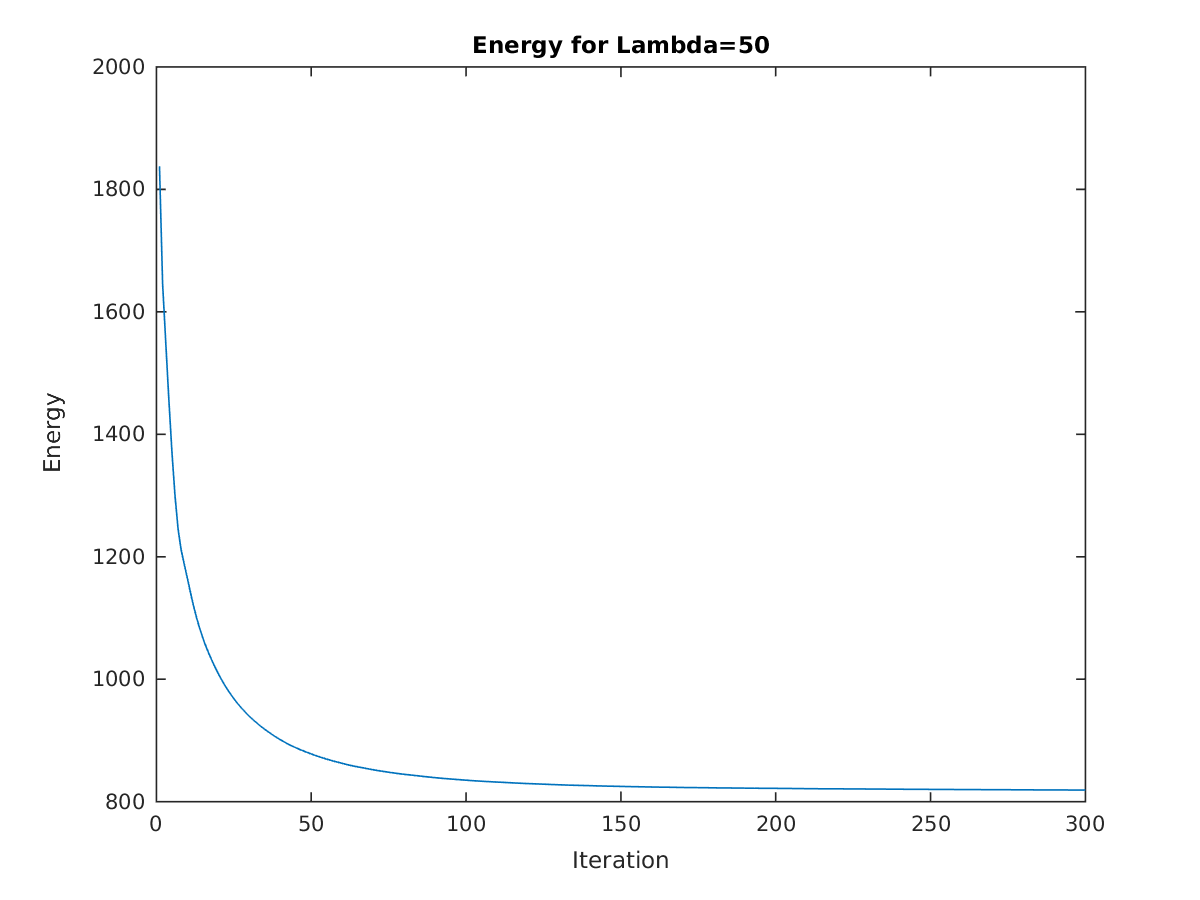
\includegraphics[width=0.45\textwidth]{energy_lambda_50.png}}
\subfigure[$\lambda = 1000$]{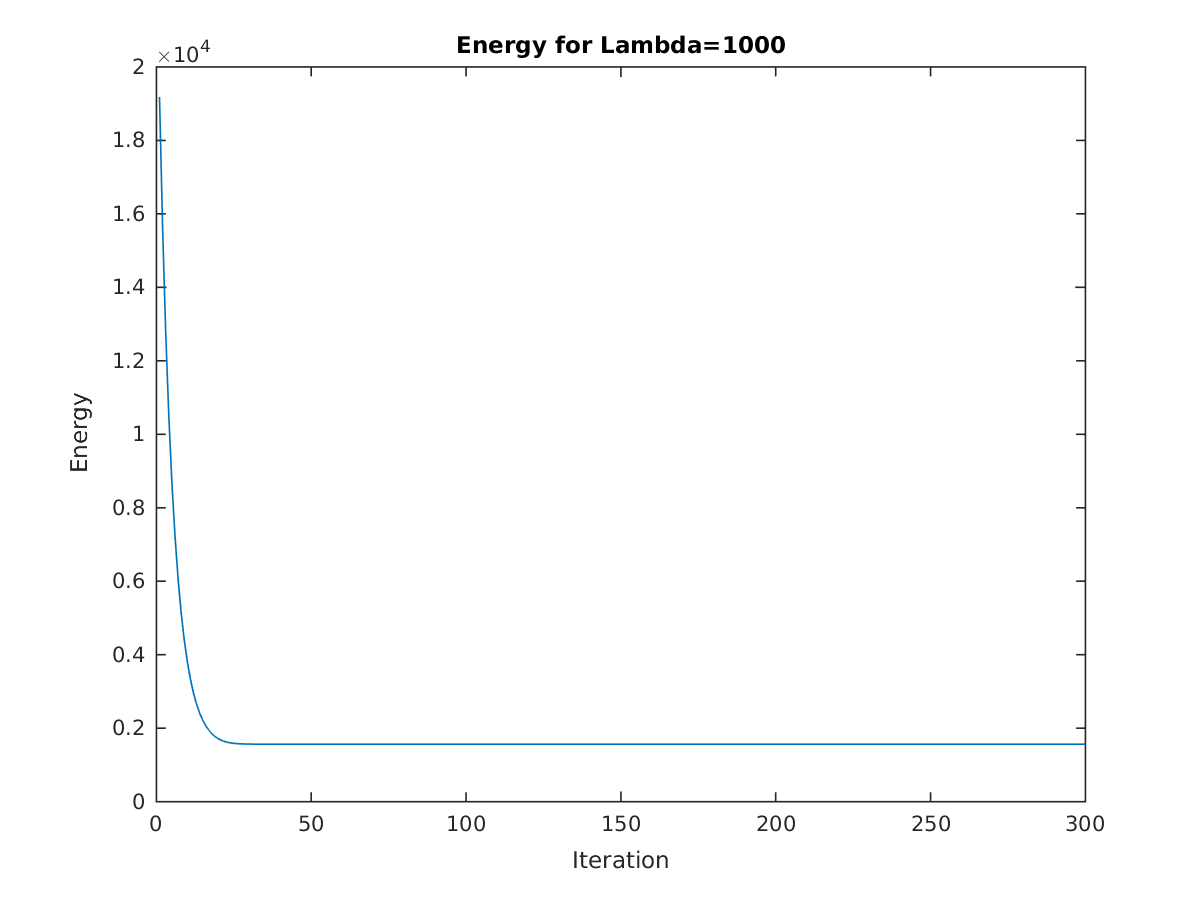
\includegraphics[width=0.45\textwidth]{energy_lambda_1000.png}} \\
\caption{Behavior of the energy function for different lambdas. For lambdas above 
a thousand, 50 iterations are enough. Smaller lambdas still improve slightly until about 300 iterations.}
\label{fig:energy_plots}
\end{figure}

\begin{figure}[ht!]%
\centering
\subfigure[0 Iterations]{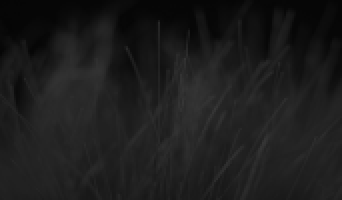
\includegraphics[width=0.32\textwidth]{grass_small_lambda_50_iteration_0.png}}
\subfigure[25 Iterations]{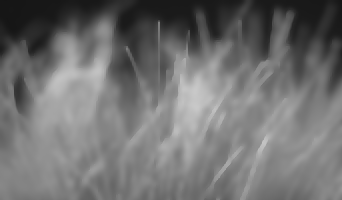
\includegraphics[width=0.32\textwidth]{grass_small_lambda_50_iteration_25.png}}
\subfigure[50 Iterations]{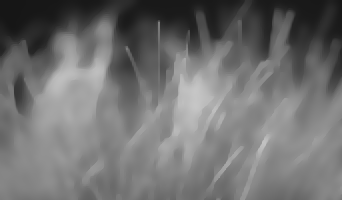
\includegraphics[width=0.32\textwidth]{grass_small_lambda_50_iteration_50.png}} \\
\subfigure[100 Iterations]{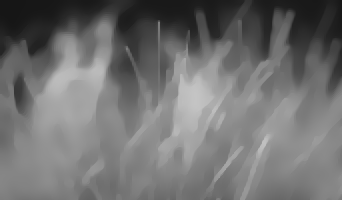
\includegraphics[width=0.32\textwidth]{grass_small_lambda_50_iteration_100.png}} 
\subfigure[200 Iterations]{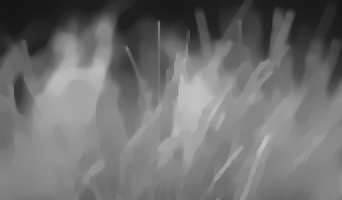
\includegraphics[width=0.32\textwidth]{grass_small_lambda_50_iteration_200.png}} 
\subfigure[300 Iterations]{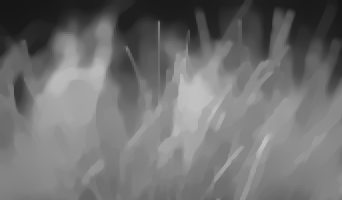
\includegraphics[width=0.32\textwidth]{grass_small_lambda_50_iteration_300.png}} 
\caption{The superresolution image after various iteration counts.
0 iterations shows the initial guess. After iteration 200 there are only
minor changes. The lambda was set to 50 for these images.}
\label{fig:iteration_count_lambda_50}
\end{figure}

\begin{figure}[ht!]%
\centering
\subfigure[0 Iterations]{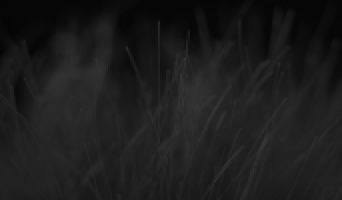
\includegraphics[width=0.32\textwidth]{grass_small_lambda_1000_iteration_0.png}}
\subfigure[5 Iterations]{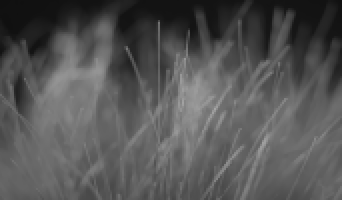
\includegraphics[width=0.32\textwidth]{grass_small_lambda_1000_iteration_5.png}} 
\subfigure[10 Iterations]{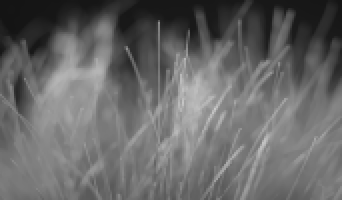
\includegraphics[width=0.32\textwidth]{grass_small_lambda_1000_iteration_10.png}} \\
\subfigure[15 Iterations]{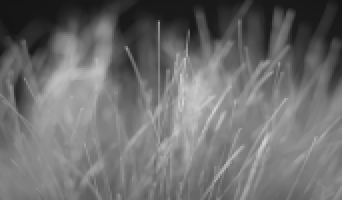
\includegraphics[width=0.32\textwidth]{grass_small_lambda_1000_iteration_15.png}}
\subfigure[20 Iterations]{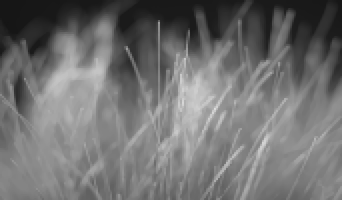
\includegraphics[width=0.32\textwidth]{grass_small_lambda_1000_iteration_30.png}}
\subfigure[300 Iterations]{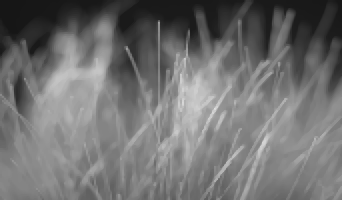
\includegraphics[width=0.32\textwidth]{grass_small_lambda_1000_iteration_300.png}} 
\caption{The superresolution image after various iteration counts.
0 iterations shows the initial guess. After iteration 30 there are only
minor changes. The lambda was set to 1000 for these images.}
\label{fig:iteration_count_lambda_1000}
\end{figure}

\subsubsection*{Effect of Lambda}
As in the previous assignment, the lambda defines the smoothness of the converged
solution. Surprisingly, I could increase lambda very high without the quality deteriorating.
With smaller lambdas ($ \lambda < 100 $), the algorithm did not converge anymore,
with default parameters, so I adapted my implementation to choose 
$\tau$ from Equation \ref{eq:tau} according to lambda:
\begin{equation}
	\tau_\lambda = 
	\begin{cases} 
		0.1 &\mbox{if } \lambda < 100 \\ 
		0.001 & \mbox{otherwise } 
	\end{cases}
\end{equation}

\begin{figure}[ht!]%
\centering
\subfigure[$\lambda = 10$]{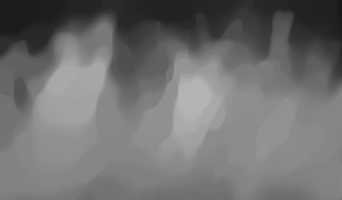
\includegraphics[width=0.32\textwidth]{grass_small_lambda_10.png}}
\subfigure[$\lambda = 100$]{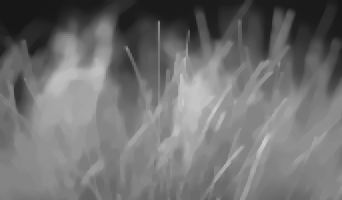
\includegraphics[width=0.32\textwidth]{grass_small_lambda_100.png}}
\subfigure[$\lambda = 1000$]{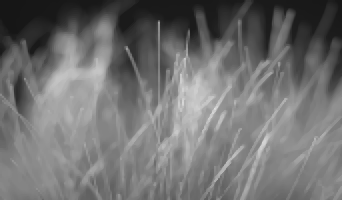
\includegraphics[width=0.32\textwidth]{grass_small_lambda_1000.png}} \\
\subfigure[$\lambda = 2000$]{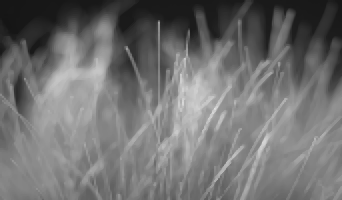
\includegraphics[width=0.32\textwidth]{grass_small_lambda_2000.png}} 
\subfigure[$\lambda = 5000$]{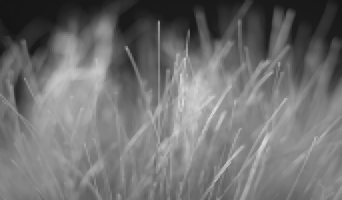
\includegraphics[width=0.32\textwidth]{grass_small_lambda_5000.png}} 
\subfigure[$\lambda = 10000$]{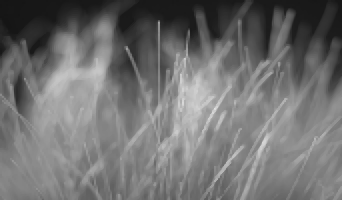
\includegraphics[width=0.32\textwidth]{grass_small_lambda_10000.png}} 
\caption{Various resulting images with different lambdas after 1000 iterations.}
\label{fig:lambdas}
\end{figure}
\clearpage

\subsubsection*{Optimal Lambda}
As already in the previous assignment, I could not find an upper bound to lambda where it starts to worsen again. But as visible in Figure \ref{fig:lambda_vs_ssd}, the SSD stays
constant after $\lambda=1000$.

\begin{figure}[ht!]%
\centering
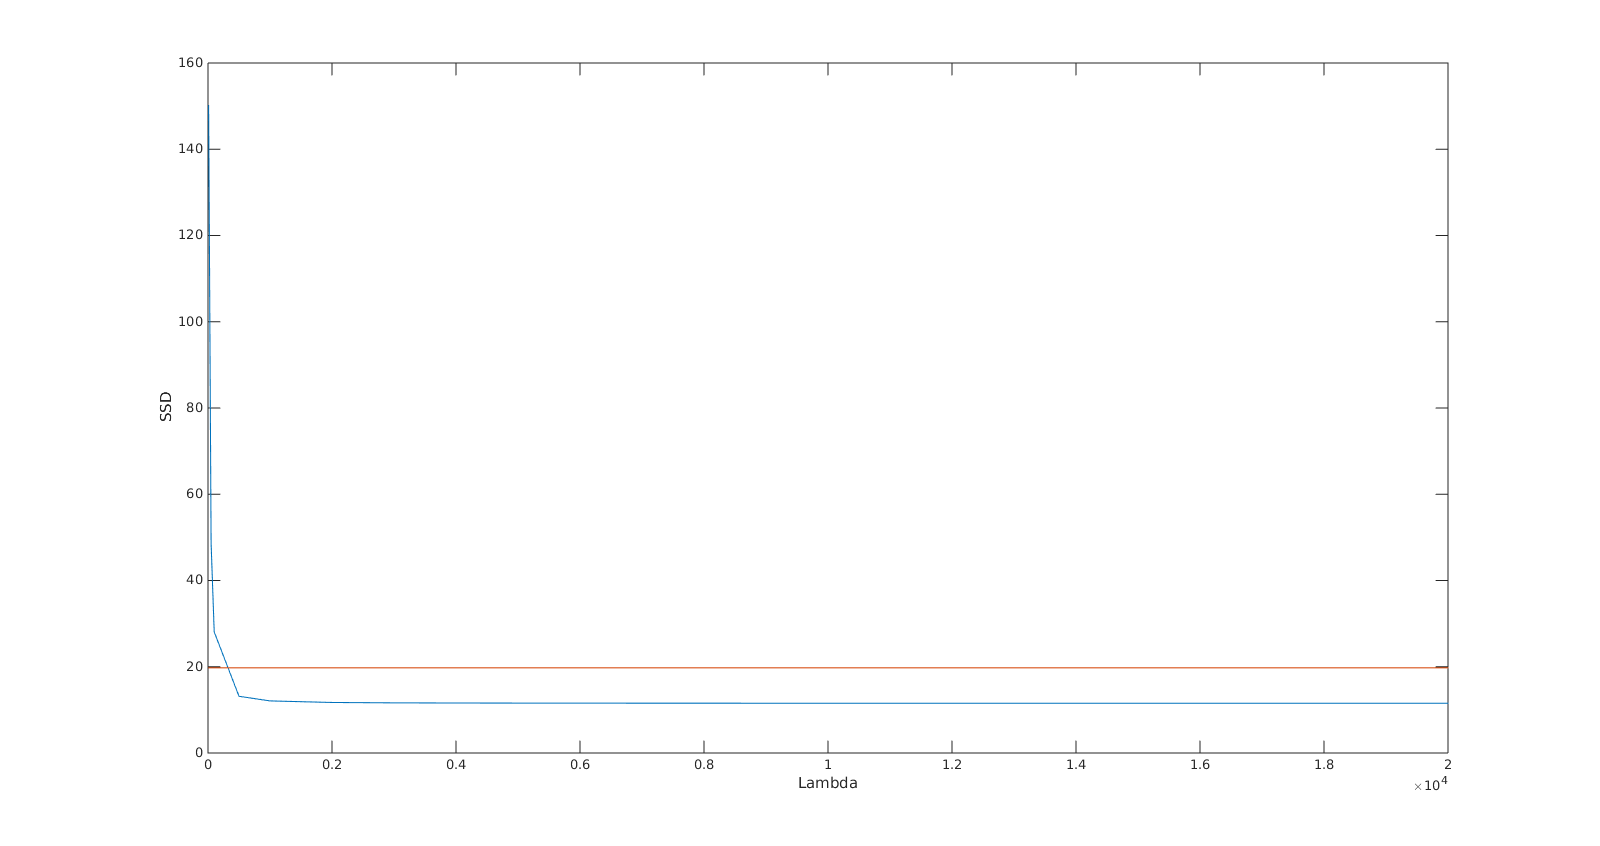
\includegraphics[width=0.9\textwidth]{lambda_vs_ssd.png}
\caption{SSD for various lambdas after 1000 iterations. For comparison, the
SSD of the image obtained through nearest-neighbor scaling was added (green line).}
\label{fig:lambda_vs_ssd}
\end{figure}

\subsection*{Conclusions}
While computational cost of one single iteration is larger is larger 
in the primal dual method, the number of iterations used until convergence 
is much lower. The convergence much trickier to achieve for the primal dual problem,
since there are more parameters to tune there. For super resolution it took 
quite some time to find acceptable values.
\end{document}
 
 